\documentclass[10pt]{article}

\usepackage[T1]{fontenc}
\usepackage{geometry}
\usepackage{amsmath, amssymb, amsthm}
\usepackage{graphicx}
\usepackage{hyperref}

\title{Probability I - Assignment II}
\author{Satvik Saha}
\date{}

\geometry{a4paper, margin=1in}
\setlength\parindent{0pt}
\renewcommand{\labelenumi}{(\alph{enumi})}
% \renewcommand\qedsymbol{$\blacksquare$}
\newcounter{prob}
\def\problem{\stepcounter{prob}\paragraph{Exercise \arabic{prob}}}
\def\solution{\paragraph{Solution}}

\begin{document}
        \par\textbf{IISER Kolkata} \hfill \textbf{Assignment II}
        \vspace{3pt}
        \hrule
        \vspace{3pt}
        \begin{center}
                \LARGE{\textbf{MA 2202 : Probability I}}
        \end{center}
        \vspace{3pt}
        \hrule
        \vspace{3pt}
        Satvik Saha, \texttt{19MS154}, Group D\hfill\today
        \vspace{20pt}

        \problem Compute the probability of obtaining a total of 10 points when two
        unbiased dice are rolled.
        
        \solution The sample space of the possible ordered rolls is given by \[
            \Omega = \{(m, n) \colon m, n \in \mathbb{N}, 1 \leq m, n \leq 6\}.
        \] Since each of the individual rolls of a die is equally likely and the die
        are independent of one another, we may write that each of the outcomes $(m,
        n)$ is equally likely. There are $6\times 6 = 36$ such tuples in $\Omega$,
        hence the probability of each of them is $1 / 36$. Note that we may set
        $\mathcal{E} = \mathcal{P}(\Omega)$. Now, we want $m + n = 10$, which is
        satisfied precisely by the tuples $(4, 6)$ $(5, 5)$ and $(6, 4)$. Hence, the
        desired probability is simply $3 / 36 = 1 / 12$.

        \problem Let $x$ be a point inside a convex quadrilateral $\mathcal{Q}$.
        Find the probability that $x$ is neither on the boundary nor inside any of
        the circles drawn with the sides of the quadrilateral $Q$ as their
        diameters.

        \solution We claim that the required probability is $0$, i.e.\ there are no
        points within $\mathcal{Q}$ which lie outside the constructed circles.  To
        show this, pick an arbitrary point $P \in \mathcal{Q}$. Draw a diagonal $AC$
        of $\mathcal{Q}$; the convexity of $\mathcal{Q}$ guarantees that the segment
        $AC$ lies entirely within $\mathcal{Q}$. Choose the triangle $\Delta ABC$ on
        the side of $AC$ where $P$ lies, or choose the vertex $B$ arbitrarily if $P$
        lies on the diagonal $AC$; thus, $P$ lies within (or on) $\Delta ABC$.
        \begin{center}
            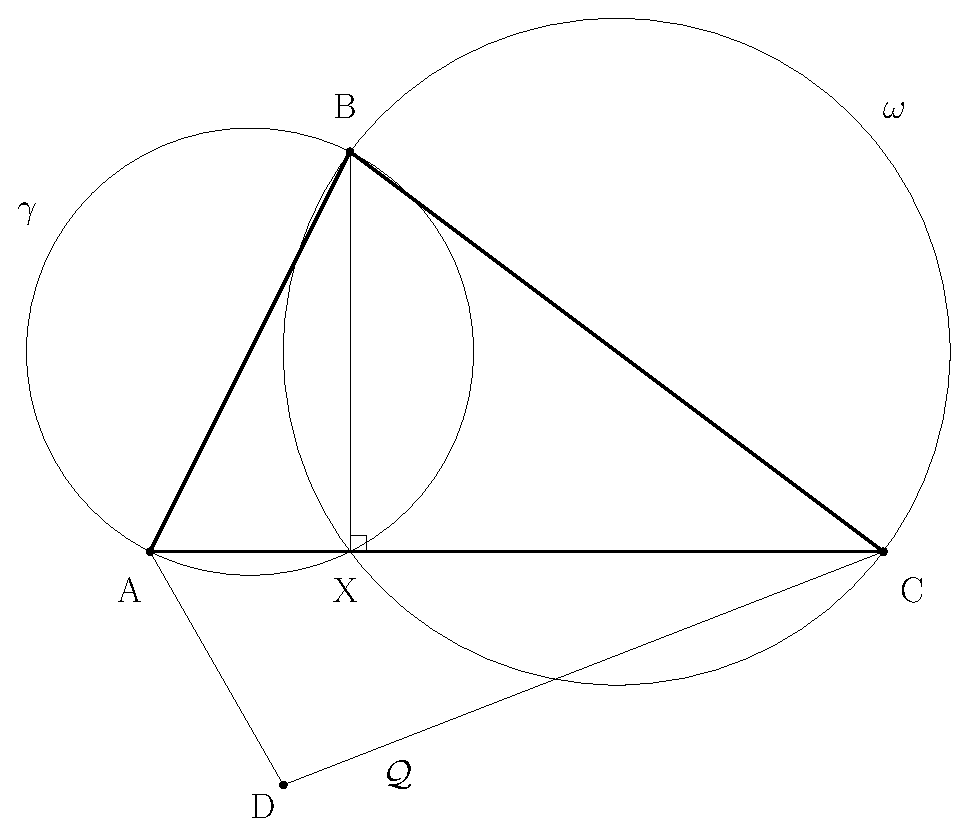
\includegraphics[scale=0.7]{./2_2_1.eps}
        \end{center}
        Now, construct a circle $\gamma$ with $AB$ as its diameter, and let it
        intersect the line $AC$ at the point $X$.  Note that the triangle $\Delta
        ABX$ is inscribed within $\gamma$, and the side $AB$ is a diameter of
        $\gamma$. This means that $\Delta ABX$ is right angled, with $\angle AXB =
        \pi /2$. Thus, $BX$ is the perpendicular through $B$ dropped on $AC$.
        Mirroring the same argument on the other side with a circle $\omega$ with
        diameter $CB$, we see that $\omega$ must cut $AC$ at the same point $X$,
        since there is only one perpendicular that can be dropped through $B$ onto
        $AC$. Thus, the triangles $\Delta ABX$ and $\Delta CBX$ both lie within
        $\gamma$ and $\omega$ (including their boundaries) so the triangle $\Delta
        ABC$ lies within the union of $\gamma$ and $\omega$. This means that $P$
        must also lie within one of the circles. Since $P$ and $\mathcal{Q}$ were
        arbitrary, there are no possible scenarios where $P$ lies outside the
        constructed circles, hence the desired probability is $0$. \\

        Note that the given argument holds even when $BX$ lies outside the triangle
        $\Delta ABC$ -- it so happens that $\Delta ABC$ is completely within one of
        the triangles $\Delta ABX$ or $\Delta CBX$. 
        \begin{center}
            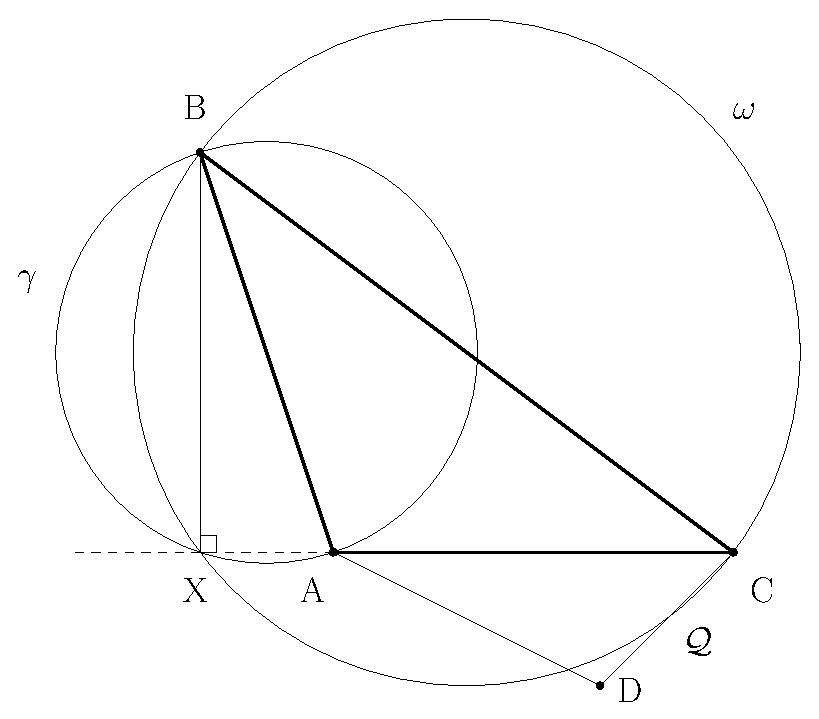
\includegraphics[scale=0.7]{./2_2_2.eps}
        \end{center}
        It also holds for any concave quadrilateral $\mathcal{Q}'$, since we can
        always draw a diagonal $AC$ lying outside $\mathcal{Q}'$; now, the entire
        quadrilateral is contained within $\Delta ABC$ where $B$ is the furthest
        vertex from $AC$, and we argue as before to show that $\Delta ABC$ lies
        within the circles constructed with $AB$ and $CB$ as diameters.

        \problem Compute the probability of getting no four consecutive heads or no
        four consecutive tails when a fair coin is tossed ten times.

        \solution Let $G_n$ denote the number of times a string of length $n$
        consisting only of the characters $H$ and $T$ which do not contain either of
        the substrings $HHHH$ or $TTTT$. Note that for $n = 1, 2, 3$, all possible
        strings of which there are $2^n$ satisfy the criterion, so $G_1 = 2$, $G_2 =
        4$ and $G_3 = 8$. \\

        Now, let $G_{n, i}$ denote that number of valid strings which end in exactly 
        $i$ identical characters. Note that \[
            G_n = G_{n,1} + G_{n, 2} + G_{n, 3},
        \] since $i = 4$ gives an invalid string. By adding another identical
        character to the end of a valid string ($H$ if the last $i$ characters were
        $H$, $T$ otherwise), we obtain $G_{n + 1, i + 1} = G_{n, i}$.  By adding the
        complementary character to the end of a valid string ($T$ if the last $i$
        characters were $H$, and vice versa), we obtain another valid string of $n +
        1$ characters with $i = 1$, so $G_{n + 1, 1} = G_{n}$.  This  gives a
        complete recursive solution : $G_{n + 3, 1} = G_{n + 2}$, $G_{n + 3, 2} =
        G_{n + 2, 1} = G_{n + 1}$ and $G_{n + 3, 3} = G_{n + 1, 1} = G_n$, so \[
            G_{n + 3} = G_{n + 3, 1} + G_{n + 3, 2} + G_{n + 3, 3} = G_{n + 2} +
            G_{n + 1} + G_n.
        \] We calculate $G_4 = 2 + 4 + 8 = 14$, $G_5 = 4 + 8 + 14 = 26$, $G_6 = 8 +
        14 + 26 = 48$, $G_7 = 14 + 26 + 48 = 88$, $G_8 = 26 + 48 + 88 = 162$, $G_9 =
        48 + 88 + 162 = 298$, $G_{10} = 88 + 162 + 298 = 548$.  Thus, there are
        $548$ valid strings out of $2^{10} = 1024$ strings of length $10$, all of
        which are equally likely to occur in a coin toss experiment.  This means
        that the desired probability is $548 / 1024 = 137 / 256 \approx 53.5\%$. \\

        \textsc{Note}:
        The sequence $G_n$ is simply twice the Tribonacci sequence $0, 0, 1, 1, 2,
        4, 7, 13, 24, \dots$, with a shift. As shown 
        \href{https://sahasatvik.github.io/kbonacci/}{here}, we can give the
        closed form expression \[
            \frac{1}{2}\, G_n = 
            \frac{\alpha^{n + 2}}{(\alpha - \beta)(\alpha - \gamma)} +
            \frac{\beta^{n + 2}}{(\beta - \alpha)(\beta - \gamma)} +
            \frac{\gamma^{n + 2}}{(\gamma - \alpha)(\gamma - \beta)},
        \] where $\alpha, \beta, \gamma$ are the roots of the polynomial $x^3 - x^2
        - x - 1$. We supply \[
            \begin{array}{rl}
                \alpha &\approx\; +1.8393, \\
                \beta  &\approx\; -0.4196 + 0.6063i, \\
                \gamma &\approx\; -0.4196 - 0.6063i.
            \end{array}
        \] Some code used for these calculations can be found
        \href{https://gist.github.com/sahasatvik/f107fe8789913954c10ecf0b56e20c52}{here}.
        \\

        The ratio $G_{n + 1} / G_n$ converges as $n \to \infty$ to the constant
        $\alpha$. This can be seen by the fact that $|\beta| < 1$ and $|\gamma| <
        1$, so the growth of $G_n$ is dominated by $\alpha^n$.  On the other hand,
        the number of strings of length $n$ grows as $2^n$. Thus, the probability of
        not getting a repeated substring of length $4$ can be made as small as we
        want, i.e.\ the probability of obtaining a stretch of $4$ identical tosses
        can be made as close to $1$ by increasing $n$.  Indeed, by $n = 30$, the
        probability of not getting a repeat is around $10\%$, and by $n = 57$, the
        probability is around $1\%$. \\

        The corresponding limiting ratio for a repeat of $k$ tosses always satisfies
        $2(1 - 2^{-k}) < \alpha_k < 2$, so the same argument above applies to show
        that we will always obtain a repeat of $k$ tosses more often than not, for a
        sufficiently high number of total tosses $n$. 
        

        \problem Let $(\Omega, \mathcal{E}, P)$ be a probability space and let $A_1,
        A_2, \dots, A_n \in \mathcal{E}$ with $P(A_1\cap \dots \cap A_n) \neq 0$.
        Show that \[
            P(A_1\cap \dots \cap A_n) = P(A_1)\, P (A_2 \,|\, A_1)\, P(A_3 
            ,|A_2\cap A_1)\, \cdots\, P(A_n \,|\, A_{n-1}\cap \dots \cap A_1).
        \] 

        \solution We prove the given statement by induction. The base case of $n =
        2$ demands \[
            P(A_1\cap A_2) = P(A_1)\, P(A_2 \,|\, A_1),
        \] which is true by definition. Note that since $P(\cap_{i = 1}^n A_i) \neq
        0$, we must have $P(\cap_{i = 1}^{m \leq n} A_i) \neq 0$ because $P(B) \leq
        P(A)$ whenever $B \subseteq A$. \\

        Suppose that the statement holds for some $n \geq 2$. Write $\cap_{i = 1}^n
        A = \mathcal{A}$, hence \[
            P(\mathcal{A} \cap A_{n + 1}) = P(\mathcal{A})\, P(A_{n + 1} \,|\,
            \mathcal{A}).
        \] Expanding $P(\mathcal{A})$ using the induction hypothesis gives the
        desired result. \[
            P\left(\bigcap_{i = 1}^{n + 1} A_i\right) = P(A_1)\, P(A_2\,|\,
            A_1)\,\cdots\, P(A_n \,|\, A_{n - 1} \cap \dots \cap A_1) \,
            P(A_{n + 1} \,|\, A_n \cap \dots \cap A_1).
        \] 


\end{document}
